\chapter{Planning with Arm-Platform Coordination for Grasp Strategies and Mobile Manipulation Tasks}
\section{Introduction}

\section{Related Work}

\section{Challenges in mobile manipulation}
All the robotic arms which are mounted on a stationary place have a limited working space. To extend the working space, mounting arms on mobile platforms is a solution. Due to the difference of mechanical 
construction of mobile manipulators, the reachability of the same manipulator can vary on different mobile platforms. Analysis of the reachability of the whole mobile manipulator can help to reason about when to use the mobile platform and how to use the mobile platform to perform manipulation tasks. In this section, we exploit a tool, capability map, originally proposed by \todo{[]}\cite{} to analyze a single robotic arm. We extend the capability of this tool to analyze the reachability of an entire mobile platform which works in a given environment. The analysis of two common manipulation scenarios reveals two big challenges in mobile manipulation. The first one is where to optimally place the mobile platform so that the working space are reachable from the arm of the robot, and also visible to the sensor of the robot. The second one is how to combine the motion of mobile platform to perform tasks in narrow working space.
  
\subsection{Reachability analysis by capability map}
A capability map is a tool to represent the reachability of a robotic arm in a given working space. The generation of a capability map requires three basic components: kinematic description of the robot, a inverse kinematic (IK) solver of the robot and a simulation environment for collision checking. The algorithm for generating the map include three steps. In the first step, a set of poses are generated systematically in the working space. To cover the entire working space of a manipulator, the working space is first discretized into a voxel grid with each voxel having the same size. In each voxel an inscribed sphere is defined. Then, a number of poses are generated evenly on the surface of the inscribed sphere. Fig.~\ref{fig:voxelgrid_sphere} depicts a set of inscribed spheres we generated for a robot. The length of each voxel is 10 cm. Fig.\ref{fig:inscribed_sphere} shows the poses generated on the surface of each inscribed sphere with different density parameters.  In the second step, the IK solver is used to compute to a solution and check the validity of the solution for all the poses. The number of the poses which have a inverse kinematic solution is recorded. This is the most time consuming step of the entire generation process. In the last step, a reachability index is computed for each voxel by 
\begin{equation}
\text{Reachability index} = \frac{ \text{Number of poses pass IK} }{ \text{Total number of poses} }   
\end{equation}

\begin{figure}[!htbp]
\centering
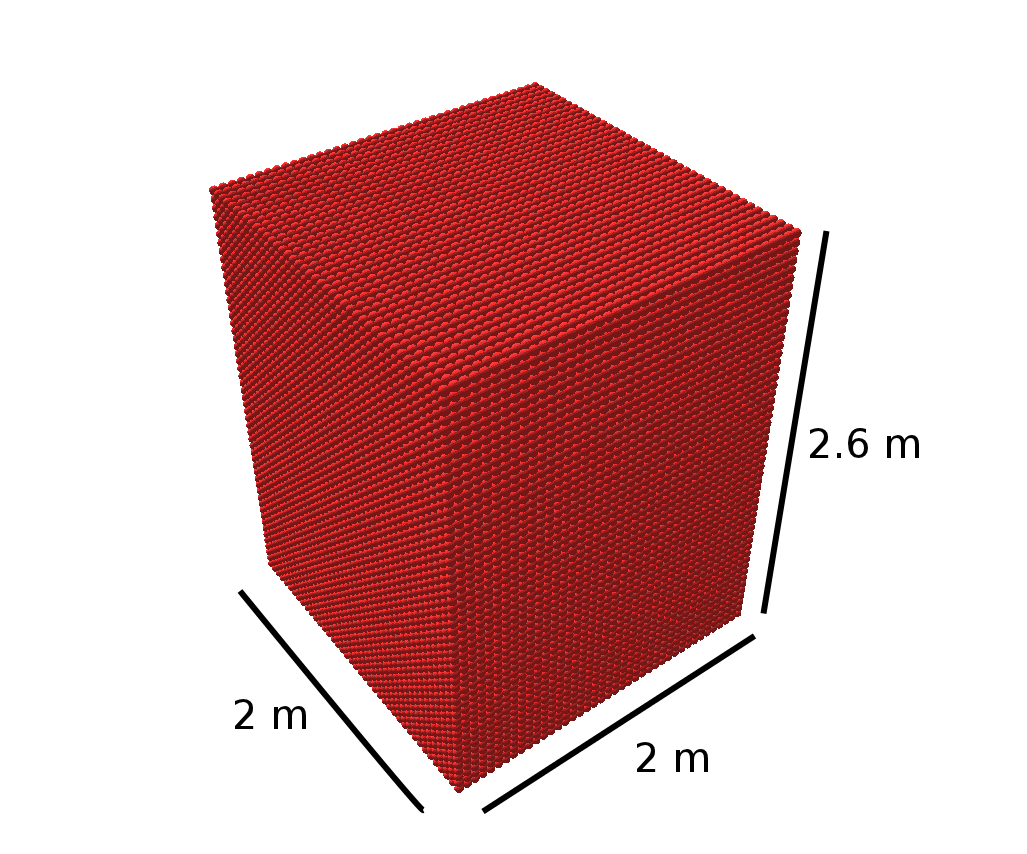
\includegraphics[width=0.6\linewidth]{voxelgridsphere.png}
\captionsetup{justification=raggedright}
\caption{A 2 m by 2 m by 2.6 m working space is discretized to voxels with the length  of each voxel equaling 10 cm. }
\label{fig:voxelgrid_sphere}       % Give a unique label
\end{figure} 


\begin{figure}[!htbp]
    \centering
    \begin{subfigure}[b]{0.25\textwidth}
        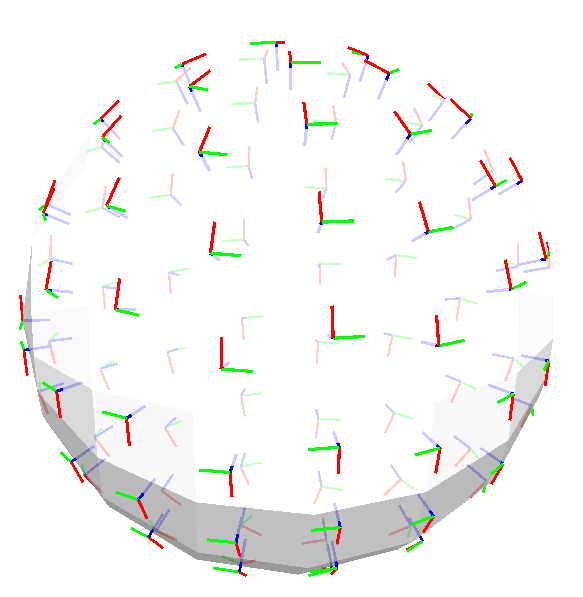
\includegraphics[width=\textwidth]{sphere100.png}
        \caption{}
        \label{fig:sphere1}
    \end{subfigure}
    ~ %add desired spacing between images, e. g. ~, \quad, \qquad, \hfill etc. 
      %(or a blank line to force the subfigure onto a new line)
    \begin{subfigure}[b]{0.25\textwidth}
        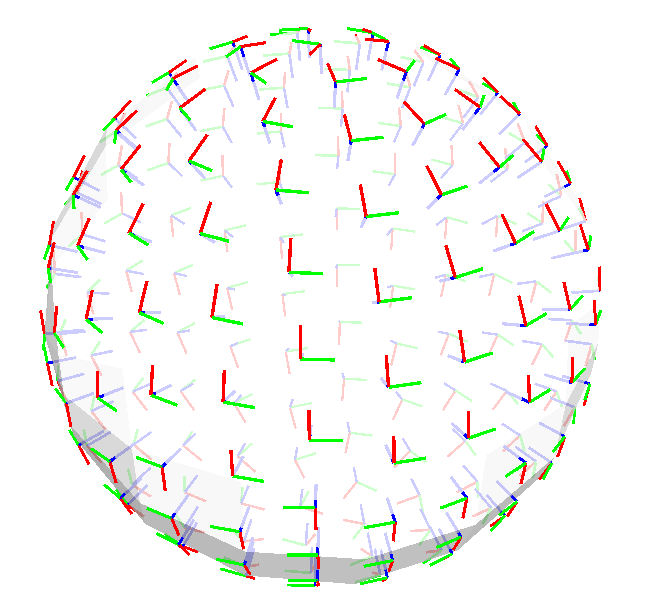
\includegraphics[width=\textwidth]{sphere200.png}
        \caption{}
        \label{fig:sphere2}
    \end{subfigure}
    ~ %add desired spacing between images, e. g. ~, \quad, \qquad, \hfill etc. 
      %(or a blank line to force the subfigure onto a new line)
    \begin{subfigure}[b]{0.25\textwidth}
        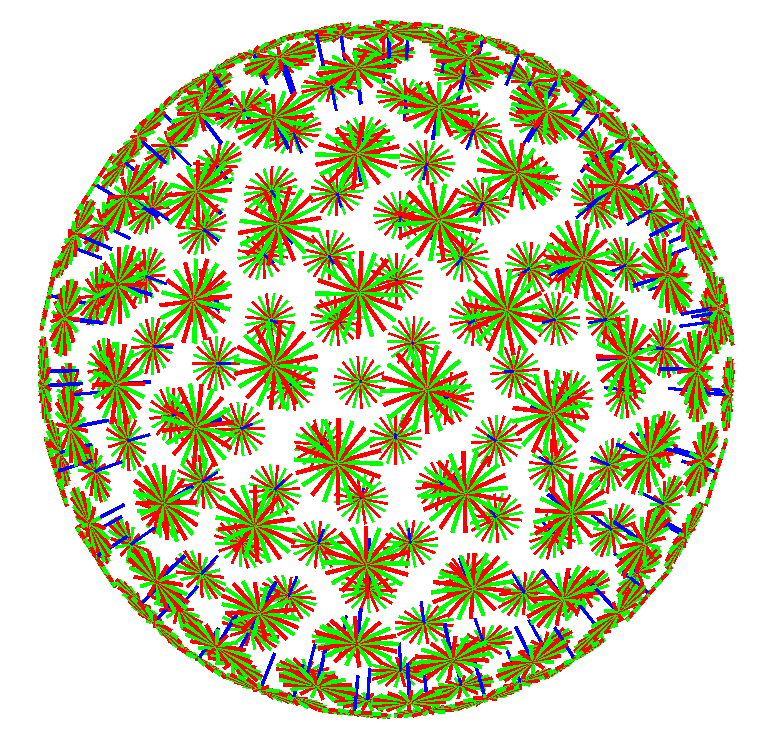
\includegraphics[width=\textwidth]{sphere3.png}
        \caption{}
        \label{fig:sphere3}
    \end{subfigure}
    \caption{Different parametrizations for generating poses on the surface of an inscribed sphere. From left to right: sparse to dense}\label{fig:inscribed_sphere}
\end{figure}

We implement the algorithm for generating the capability map in the OPENRAVE \todo{\cite{}} simulator. The IK-FAST inverse kinematic solver is chosen to compute  whether a solution exists or not. An extension to this implementation is that we can include additional environment models in the simulator so that a collision checker provided from the simulator can be used to rule out the IK solutions which contain self collisions or collisions with environment. Fig.~\ref{fig:cmap} depicts the capability map at the height of 0.75 m. We parametrize 200 poses to be generated on each inscribed sphere. The total time for generating the map is about 30 minutes. The maximal reachability index of the manipulator is about 85 \%. Fig.~\ref{fig:cmap_view1} and Fig.~\ref{fig:cmap_view2} illustrate a side-view and a top-view of the capability map respectively. The region occupied by the magenta spheres are the optimal place which grasp or manipulation tasks should be conducted, because in these places the manipulator has the largest reachability index. 

\begin{figure}[!htbp]
\centering
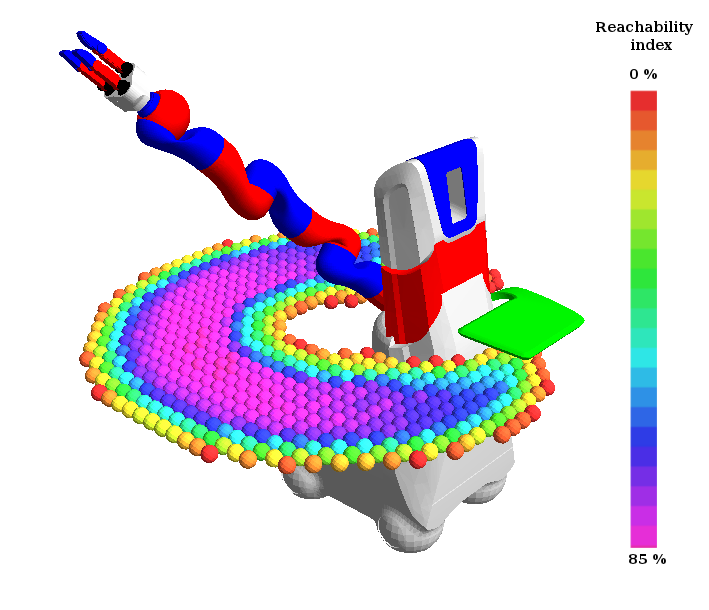
\includegraphics[width=0.7\linewidth]{reachability_map_table_with_index.png}
\captionsetup{justification=raggedright}
\caption{Visualization of a capability map at the height  of 0.75 m. The magenta spheres indicate the region where the manipulator has the largest manipulability.}
\label{fig:cmap}       % Give a unique label
\end{figure} 

\begin{figure}[!htbp]
    \centering
    \begin{subfigure}[b]{0.45\textwidth}
        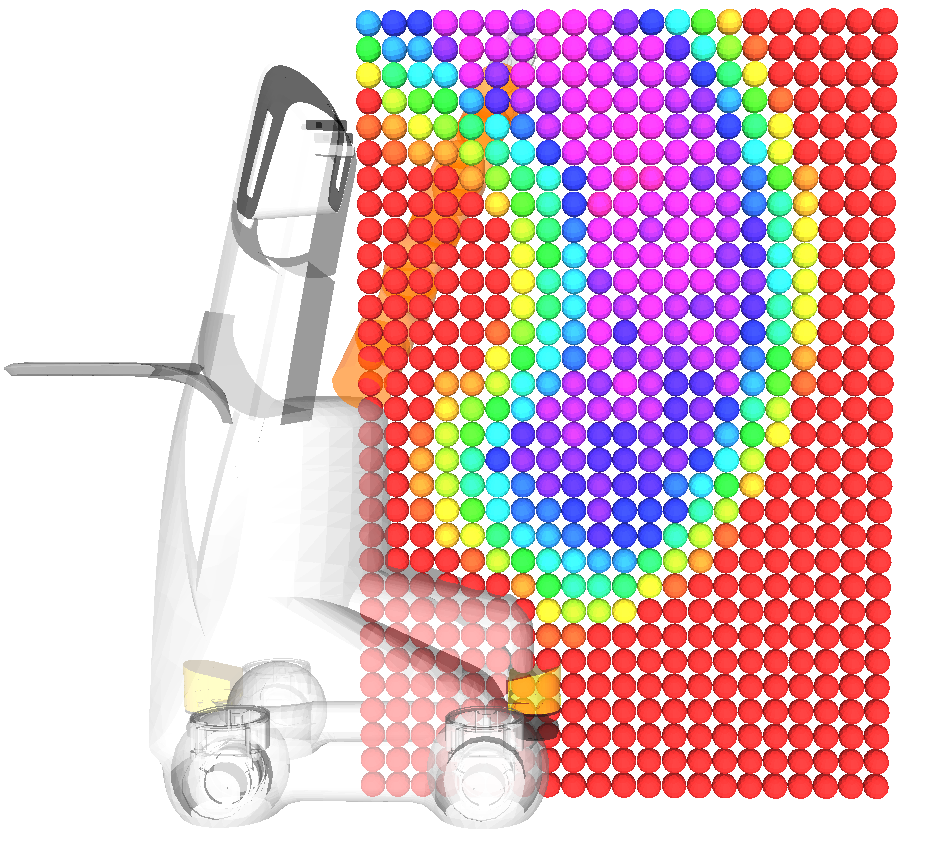
\includegraphics[width=\textwidth]{capability_robot_alone.png}
        \caption{A cross section visualization in XZ plane viewing from the side of the robot. }
        \label{fig:cmap_view1}
    \end{subfigure}
    ~ %add desired spacing between images, e. g. ~, \quad, \qquad, \hfill etc. 
      %(or a blank line to force the subfigure onto a new line)
    \begin{subfigure}[b]{0.45\textwidth}
        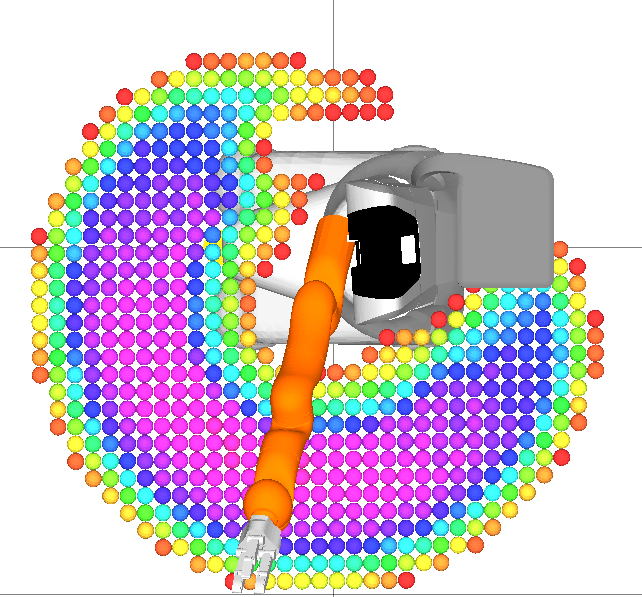
\includegraphics[width=\textwidth]{reachabilityz075.png}
        \caption{A cross section visualization in XY plane viewing from the top of the robot. }
        \label{fig:cmap_view2}
    \end{subfigure}
    \caption{ A cross-section visualization of the capability map from two perspectives. }\label{fig:cmap_view}
\end{figure}

%\subsubsection{Step 2: Run IK solver on all the poses}

%\subsubsection{Step 3: Extract reachability index}

\subsection{Analysis of two common manipulation scenarios}
So far we gave a brief introduction to the capability map and how to use this tool to inspect the reachability of a mobile manipulator. In this section, we analyze two common manipulation scenarios. The result indicate two major challenges that exist in the context of mobile manipulation.  

\subsubsection{Challenge 1: Optimal placing of a mobile manipulator}

The first scenario we consider is manipulation on table-tops. In this scenario, a robot grasps, places and manipulates objects above a table-top. We include a box to represent the collision model of a table and place a robot in front of it. Two capability maps are generated by placing the robot at two different distance. Fig.~\ref{fig:cmap_tables} depicts the results. The number of magenta spheres above the table in Fig.~\ref{fig:cmap_table1} is more than in Fig.~\ref{fig:cmap_table2}. This indicates that the closer we place the robot to the table, the more region the robot can reach. This phenomena is in accordance with the intuition. However, if we consider the field of view of the sensor which is mounted on the head of the robot simultaneously, placing a robot as close as possible to the table is not the optimal solution. In this case the object to be grasped (marked in red) could lie outside the field of view of the sensor, so that the robot can not locate the object at all. Furthermore, the problem also exists in the opposite situation. Fig.~\ref{fig:cmap_table2} demonstrates the opposite situation. The robot is placed farther to the table comparing with in Fig.~\ref{fig:cmap_table1}. The region above the table can be covered by the complete field of view of the sensor. The robot is able to locate the object at this distance, however the manipulator of the robot can not reach the table as shown from the capability map. Although we demonstrate the problem with a fixed head-mounted camera, the problem also exists for an eye-in-hand configuration (sensor attached to the end effector). The capability map, which combines a given environment model in computation,  reveals the first challenge we want to address in the mobile manipulation: where to place the robot so that the grasping and manipulation tasks can be performed. 

\begin{figure}[!htbp]
    \centering
    \begin{subfigure}[b]{0.37\textwidth}
        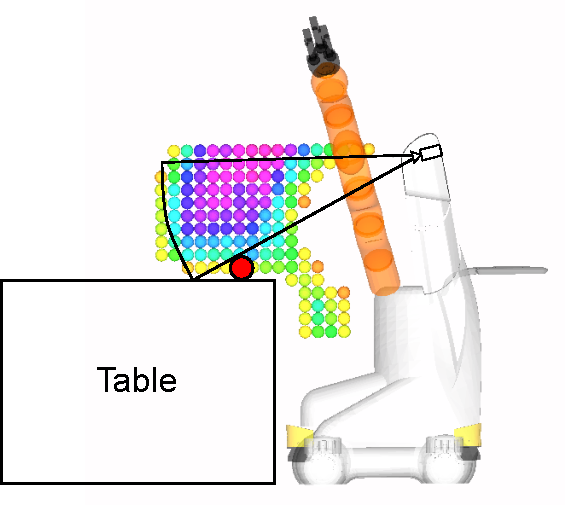
\includegraphics[width=\textwidth]{reachability_table1.pdf}
        \caption{The object lies outside the FOV of the sensor, when placing the robot too close to the table.}
        \label{fig:cmap_table1}
    \end{subfigure}
    ~ %add desired spacing between images, e. g. ~, \quad, \qquad, \hfill etc. 
      %(or a blank line to force the subfigure onto a new line)
    \begin{subfigure}[b]{0.45\textwidth}
        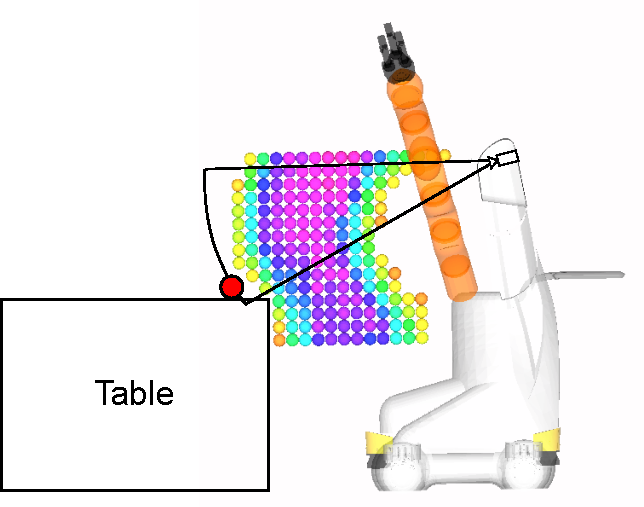
\includegraphics[width=\textwidth]{reachability_table2.pdf}
        \caption{The object is not reachable from the manipulator when placing the robot too far to the table.}
        \label{fig:cmap_table2}
    \end{subfigure}
    \caption{Captability maps generated for two configurations of the robot}\label{fig:cmap_tables}
\end{figure}

\subsubsection{Challenge 2: Planning motion in limited working space} 

The second challenge for the mobile manipulation is how to grasp the objects in narrow working space. We select picking from a shelf as an example scenario to demonstrate the challenge, since this task is a common scenario in human environments. We configure the simulation by placing the robot in front of a shelf model. The capability map is generated for the entire working space inside the shelf model. A cross section visualization of the capability map in this environment is given in Fig.~\ref{fig:cmap_shelf}. The maximal reachability index of this environment is only about 20\%. This not only means the number of reachable poses inside the shelf is very low, but also indicates that the valid configuration space, in which the manipulator does not collide with the shelf,  is very limited. Although the manipulator can reach inside the shelf, it may be difficult for a motion planner to plan a collision-free path to reach inside the shelf. To verify this problem, we construct a planning scenario in Moveit \todo{[]}\cite{} and benchmark the success rate of motion planning in this environment. We use one start configuration and four goal configurations to conduct the benchmarking (see Fig.~\ref{fig:moveit_planning}). Three motion planners are used for comparison. They are RRT-connect, Probabilistic Roadmap Method (PRM) and Expansive Space Trees (EST). For each configuration, 10 planning queries are conducted for each planner. Table.~\ref{tab:benchmark_result} gives the success rate for each configuration/planners. The overall success rate of motion planning in this limited working space is only 26 \% in spite of all the configurations are reachable by the manipulator. The result of the benchmarking explains use the manipulator alone is not the solution  for mobile manipulators to work in a limited environment. The mobility of the robot has to be considered with the manipulator together to overcome the problem. The challenge remains how to exploit and combine the mobility to allow a robot still be able to  work in such narrow environments. 

\begin{figure}[!htbp]
\centering
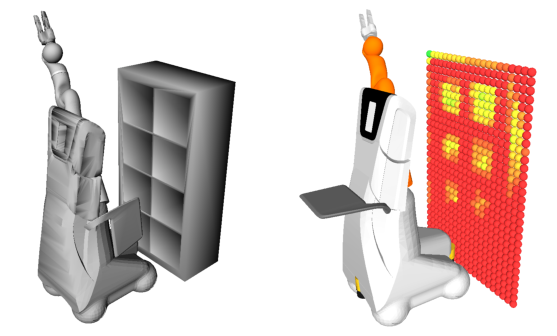
\includegraphics[width=0.7\linewidth]{reachability_shelf.pdf}
\captionsetup{justification=raggedright}
\caption{Capability map generated for picking-from-shelf scenario. }
\label{fig:cmap_shelf}       % Give a unique label
\end{figure} 

\begin{figure}[!htbp]
\captionsetup[subfigure]{position=b}
    \centering
    \begin{subfigure}[t]{0.18\textwidth}
        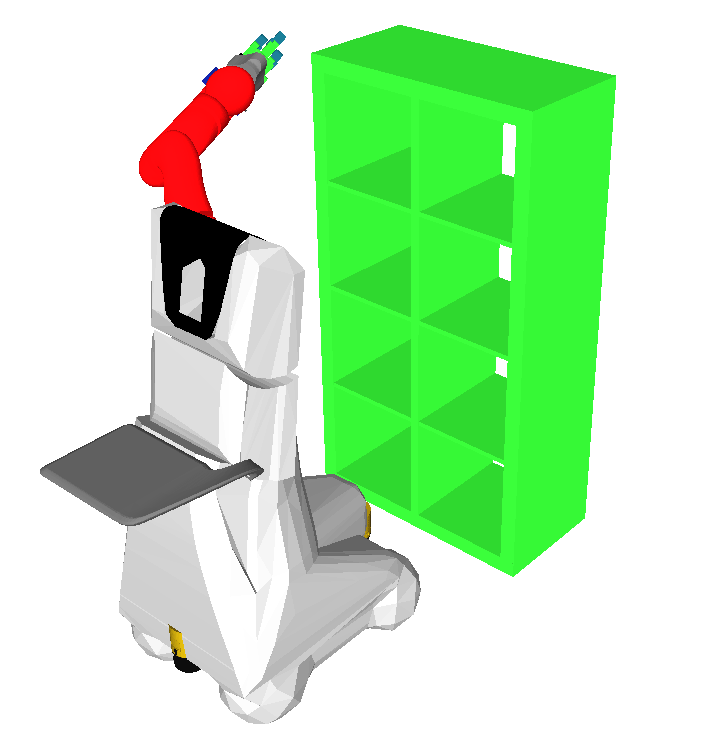
\includegraphics[width=\textwidth]{start_state.png}
        \caption{Start configuration }
        \label{fig:start_state}
    \end{subfigure}
    ~ %add desired spacing between images, e. g. ~, \quad, \qquad, \hfill etc. 
      %(or a blank line to force the subfigure onto a new line)
    \begin{subfigure}[t]{0.72\textwidth}
        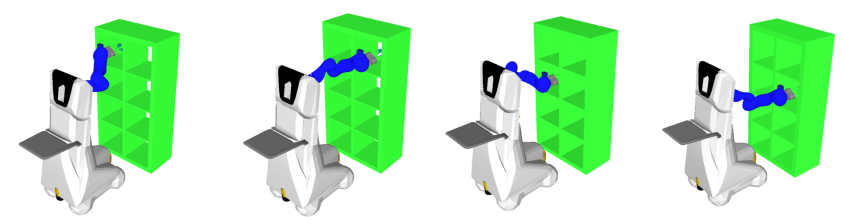
\includegraphics[width=\textwidth]{goal_states.pdf}
        \caption{Goal configurations}
        \label{fig:goal_states}
    \end{subfigure}
    \caption{Start and goal configurations for benchmarking the motion planners in a limited working space.}\label{fig:moveit_planning}
\end{figure} 

\begin{table}[!htbp]
\centering
\begin{tabular}{lrrrr|r}
Planner     & goal 1 & goal 2 & goal 3 & goal 4 & Average \\ 
\hline
\hline
RRT-Connect & 40\%   & 100\%  & 40\%   & 10\%   & 47\%    \\
PRM*        & 10\%   & 60\%   & 0\%    & 10\%   & 20\%    \\
EST         & 10\%   & 40\%   & 0\%    & 0\%    & 12\%    \\ \hline
Overall     &        &        &        &        & 26\%   
\end{tabular}
\caption{Planning success rate of three state-of-the-art motion planners in terms of 4 different goal configurations. 10 planning queries are conducted for each goal configuration to compute the statistic. In summary, 120 planning queries are conducted for the given scenario, only 26\% overall success rate is achieved by the planners. } 
\label{tab:benchmark_result}
\end{table}

\section{Model arm-platform coordination}

\subsection{Model platform's DoF as virtual Joints}

\section{Design of grasp strategy for pre-grasp phase}

\subsection{Strategy definition}
 
\subsection{Active interaction strategy for model-based objects}

\subsubsection{Strategy selection etc.}

\section{Planning for mobile manipulation tasks}
\subsection{Task definition}
\subsection{Base position planning}

